\documentclass[a4paper,11pt]{article}
\usepackage{amsmath}
\usepackage{listings}
\usepackage{enumerate}
\usepackage{graphicx}
\usepackage{hyperref}
\usepackage[font=small,labelfont=bf]{caption}
\usepackage{geometry}


\title{House Price Prediction}
\date{March 30, 2019}
\author{Lucas Faijdherbe, Rico Mossinkof, Ewoud Vermeij, Ruben van der Ham\\ and Harsh Khandelwal\\\\
\small Machine Learning\\
\small Vrije Universiteit Amsterdam}

\begin{document}
\maketitle

\pagenumbering{arabic} %pagenumbering ON


\begin{abstract}
The aim of this report is to predict the house prices for houses in Ames, Iowa. House price predictions are made using a dataset which includes 79 features per house. Two different classes of machine learning models will be used, k-nearest neighbours and linear regression. Our results show that there is only a small difference between the performance of the k-NN and the linear regression. Both perform better than the baseline model, which is a random predictor. As the difference between the linear regression and k-NN is minimal, we cannot conclude that there is a model that is better in the prediction of house prices. Future research could focus on a creating more versions of these models to compare the performance.
\end{abstract}

\section{Introduction}
After the downfall of house prices in the Netherlands during the economic recession, prices are starting to rise again. In some areas the house prices are rising with a tremendous pace. A good example is Amsterdam, where house prices rose with a staggering 20\% in one year [1]. Fluctuations in house prices are not only interesting for potential house owners, but also for investors, which are partial responsible for the upswing in house prices [2]. This makes house price prediction an interesting topic. \\ 
\indent The data used for the training and testing of the prediction algorithms came from kaggle.com from a competition called “House Prices: Advanced Regression Techniques”. The dataset provided for this competition contains the features of residential homes of Ames, a small town in Iowa, United States. It has to be noted that a potential model that is able to predict the house prices of this dataset is unlikely to have the same performance on a dataset of a different residential area. Nonetheless it is a great dataset to use for this research. The goal is to be able to have a model that can accurately predict the house prices for this dataset. \\
\indent There have been several approaches for predicting or evaluating house prices. The hedonic-based regression is one approach. With hedonic-based methods, relationships between house prices and house characteristics are tried to be identified. This has been utilized in many reports [5][6][7].  Besides hedonic-based regression, there have been several approaches in the machine learning area. Interestingly we found that these approaches are not necessarily complex ones. Use of a decision tree is a relatively simple approach, but can get a descent squared error rate such as 0.885 [3]. It is also shown that an algorithm like RIPPER, a rule-learning algorithm, can outperform slightly more complex algorithms such as Naïve Bayesian and AdaBoost [4]. Therefore this report is focused more on investigating the performance among relatively simple algorithms.  \\ 
\indent The focus will be on two different machine learning techniques: linear regression and k-nearest neighbours. According to earlier research [12],  k-nearest neighbours (k-NN) can have some promising results when it comes to house price prediction. For linear regression no relevant research was found, so this paper will try to investigate its performance. It is expected that k-NN will be relatively accurate. To compare the results a baseline model is used. This baseline predicts every house price with the average of all house prices. The models laid out in this report should perform better than this baseline model, as the average will not give a very good prediction. \\
\indent The following of the report is structured as follows. Section 2 will talk about the analysing of the dataset, and discuss the data preparation. Section 3 will discuss the models individually. Section 4 will present the experimental results and concluding remarks on the results. 


\section{Data analysis and preparation}
In order to get the best performance from the machine learning models, the dataset features need to be analysed and prepared such that the models can work with the data and will be able to make predictions based off of it. \\
\indent The first section will take a closer look at all features to get a good understanding of how all data is distributed, how it is presented (numerical or categorical) and if any data is missing. The next section will elaborate on the data preparation decisions made in order to get the best results with the models.


\subsection{Data Analysis}
The dataset provided through the kaggle competition consists of 79 features describing the residential homes from Ames, Iowa. The kaggle competition provided two datasets: one to train on and one to predict from. However, the prediction data set does not include the actual house prices. It is not possible to use this dataset, since there will be no way to check if the model prediction performed well on this data. Only the ‘train’ dataset will be used, which will be split randomly in a train and test set. This dataset consists of 1460 entries. \\
%figuur sale price
Since sale price is the target to predict, let us look how the sale price relates to other properties. Figure 1 shows that the sale price looks like a right skewed normal distribution. Most of the sale prices lie around 180.921 dollars. This is the mean of the data and this will be used for the baseline. \\
%figuur heatmap
Figure 2 shows a heatmap which shows the correlation between 40 of the features, including the sale price. This can be very valuable information. Features with little or close to zero correlation with respect to the sale price could be left out from training a model, since they do not say much about the sale price. On the other side, features with high correlation with the sale price are valuable. Putting the emphasis on these features when training the models can be meaningful. //

Figure 3 shows a table of the six features having the highest fraction of missing values. In some situations it can be in helpful to delete the rows containing missing value(s) for one or more features. In this situation, this is not a viable option since 99.5\% of the rows have no value for the pool quality.

%figuur 3 feature percent missing


\subsection{Data Preperation}
In order to make the data useable for the models, some enhancements need to be made. Since the sale price data was somewhat skewed, log transformation was performed in order to normalise it. For categorical features that missed entries (e.g. entries containing NA), the entries were filled. As an example, for the feature “central air conditioning”, all the missing entries were assumed to a NO, since there are only two possibilities, a YES and a NO. Some categorical features containing numerical values were changed to numerical features. An example is garage quality, where the conditions ranged from poor to excellent. These can be easily changed into numerical features. However, these changes do not always work out well so in some cases the numerical features had to be changed back to categorical features. \\
\indent Next, missing values for numerical features were handled by taking the mean of the feature as a replacement. The numerical features that were skewed were also log transformed, in order to normalise them. For categorical features one-hot coding was applied, in order to only have numerical features in the feature space. In the end, the correlation between features and sale price was plot again. The 80 highest correlated features with respect to the sale price were taken. The other features were discarded. These discarded features were the most ‘meaningless’, so the model should perform better since the decisions will be based on more highly correlated features. 


\section{Evaluated Models}
\subsection{Linear Models}
Linear Regression can model all the input variables to the house price, and can make predictions based of this model. Linear Regression will try to find the best fitting line for the model. To help fit the model, we performed regularization. This is a technique to reduce the magnitude of the coefficients, in order to lessen the impact of some very high coefficients on the model. This can help against overfitting. We looked at both LASSO (LL(1)) [9] and Ridge (LL(2)) [10] regularization, but opted to go for LASSO since it performed slightly better on our variables. What LASSO does is add a penalty term that changes depending on the alpha value. The higher the alpha, the higher the penalty and the more the variables are impacted. Ridge does this as well, but LASSO is a bit more aggressive, because even for small alphas, a lot of variables will be reduced to 0. This is called feature selection.  The LASSO regularization technique removed 118 features from our model. 

\subsection{K-nearest neighbours}
K-nearest neighbours (k-NN) is a simple, straightforward, lazy classifier. This classifier determines a certain point by looking at the k nearest points, which have been already classified. k-NN can be used for classification and regression. For the house price prediction a regression variant is used, where k-NN looks at his k closest neighbours and takes the mean of the sale price of those neighbours to determine the price. To retrieve the best model, the k for for which the model will perform best needs to be determined. Picking a low k tends to overfit the model. Picking a high k will increase bias and lowers variance. A rule of thumb can be used to determine k, which is $\sqrt{n}$ where n is the size of the dataset [8]. \\
\indent To determine the best model, grid search [11] was used, in combination with k-fold cross validation. This makes an efficient look for the hyperparameters of the best performing model possible. A 4-fold cross validation was used, where 3 groups are the training set, and 1 group is the validation set. A larger fold would not be feasible, since there are only 1460 data entries. The grid search algorithm will be run with different ranges for k. Section 4 will elaborate on the performances of different k’s, which will be measured with the mean squared error. 

\section{Results and conclusion}
To compare the models performance of k-NN and Linear Regression four different metrics are used: Mean Squared Error (MSE), Median Absolute Error (MAE), $R^2$  and Variance Score (VS). MSE subtracts each true value from the predicted value, squares it and sums them up to one value. This value gets divided by the number of samples used for this test. The lower the score, the better. Mathematical notation:
\\

\begin{center}
$MAE(xPred,yTrue)=median(|ytrue_1-xPred_1|,....,|yTrue_n-xPred_n|)$
\end{center}

With VS, we mean the explained variance score. This score measures the proportion to which the model accounts for the variation of the dataset. The higher the score, the better. Mathematical notation:
\\

\begin{center}
$VS(xPred,yTrue)=\frac{1-Variance\{yTrue-xPred\}}{Variance\{yTrue\}}$
\end{center}

With these four metrics we will evaluate the KNN models with the Linear models in the next section.

\subsection{Results}
In the table below we can see the results of KNN for different values of K. The first thing we notice is the relatively small difference in performance for different values of K. In section 3.2 we also stated that a good value for K is $\sqrt{n}$ with n the number of samples in the dataset. $\sqrt{1460}\approx38$, but as we can see, high values of K give a slightly worse performance compared to lower values of K. We suspect the small performance difference being caused by the distribution of the house prices. As we saw in section 2.1, most houses have a value between 100,000 and 200,000. For lower K we have a better score, because a higher K will predict closer to the mean of all house prices.

\clearpage
\begin{table}[]
\centering
\begin{tabular}{|l|l|l|l|l|}
\hline
\textbf{K} & \textbf{MSE} & \boldmath{$R^2$}  & \textbf{MAE} & \textbf{Variance Score} \\ \hline
1          & 0.04438      & 0.67318     & 0.12382      & 0.67551                 \\ \hline
2          & 0.03633      & 0.72176     & 0.10237      & 0.72523                 \\ \hline
3          & 0.03293      & 0.73254     & 0.10567      & 0.7379                  \\ \hline
5          & 0.03381      & 0.71273     & 0.09867      & 0.72034                 \\ \hline
10         & 0.03409      & 0.68273     & 0.09593      & 0.69413                 \\ \hline
20         & 0.03482      & 0.64114     & 0.09353      & 0.65419                 \\ \hline
30         & 0.03525      & 0.61532     & 0.09076      & 0.62779                 \\ \hline
40         & 0.03619      & 0.58598     & 0.09773      & 0.59754                 \\ \hline
\end{tabular}
\caption{KNN hyperparameter K performance}
\end{table}

\begin{table}[]
\begin{tabular}{|l|l|l|l|l|}
\hline
\textbf{Model}                  & \textbf{MSE} & \boldmath{$R^2$} & \textbf{MAE} & \textbf{Variance Score} \\ \hline
Basic Linear Regression Model   & 0.020639                    & 0.868137    & 0.068745                       & 0.861218                \\ \hline
L1 Regularized Regression Model & 0.020402                    & 0.868323    & 0.071037                       & 0.862814                \\ \hline
L2 Regularized Regression Model & 0.020372                    & 0.869291    & 0.06878                        & 0.863015                \\ \hline
KNN (gridsearch) with K = 3     & 0.03293                     & 0.73254     & 0.10567                        & 0.7379                  \\ \hline
Mean house price                & 0.15454                     & -4.89788    & 0.26358                        & -4.71305                \\ \hline
\end{tabular}
\caption{Comparison of models}
\end{table}







\section{Conclusion}
Our baseline has some divergent results. Both $R^2$ and the variance are negative scores. 
All of our models have a significantly better performance than the baseline model. This means that they have actually learned how to predict the prices instead of just randomly guessing it. Inbetween the models there are some interesting relations. There doesn’t seem to be much difference between the linear models with and without regularization. This may be the case because the linear model is not overfitting. In this case regularization would indeed not be very useful. It is also possible that our model is overfitting, but the predicted prices are still quite accurate. Because most of the house prices lie in the same price range, it could still predict most of the prices around their actual price. 
Overall, the linear regression models seem to perform slightly better than the knn model.  Because most of our data has a sale price around the mean, linear regression actually predicts the sale price quite accurate. Knn still has a good performance compared to the baseline,  with approximately 5 times less (mean squared) error.






\section*{LATEX EXAMPLE STUFF LEAVE IT HERE}


\begin{center}
\begin{minipage}{0.49\linewidth}
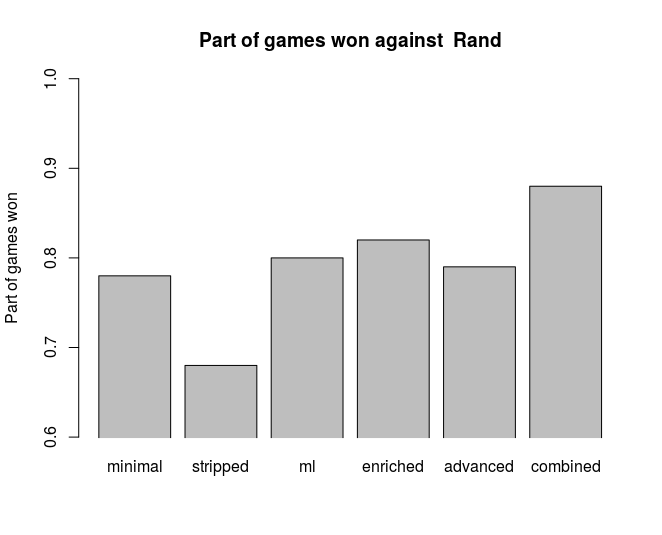
\includegraphics[width=\linewidth]{images/barplotRand.png}
\captionof{figure}{Part of games won against Rand}
\end{minipage}
\hfill
\begin{minipage}{0.49\linewidth}
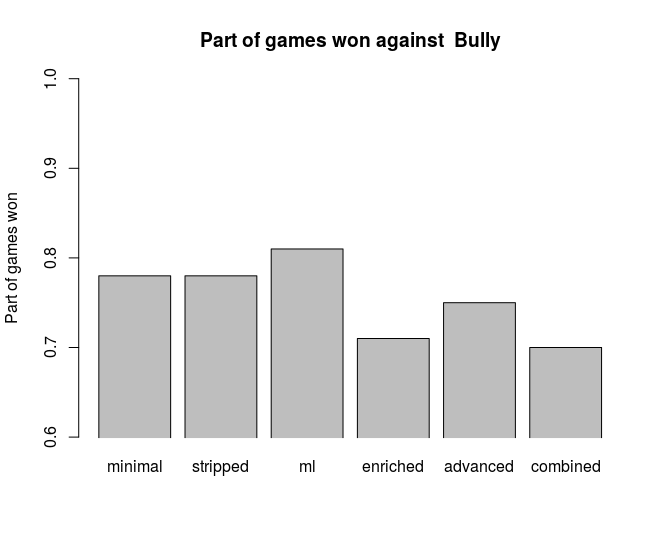
\includegraphics[width=\linewidth]{images/barplotBully.png}
\captionof{figure}{Part of games won against Bully}
\end{minipage}
      \\ %extra line for space
\begin{minipage}{0.49\linewidth}
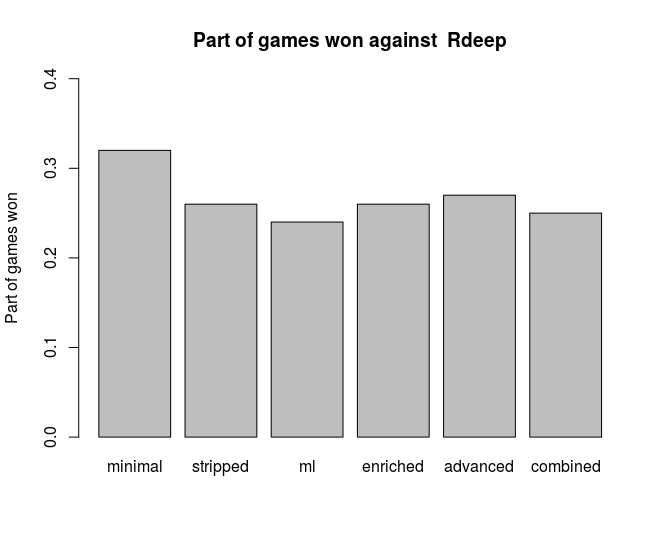
\includegraphics[width=\linewidth]{images/barplotRdeep.png}
\captionof{figure}{Part of games won against Rdeep (mind the different Y-axis)}
\end{minipage}
\end{center}
\clearpage
\section{Findings}

\subsection*{Against Rand}
There are a few notable things when comparing the performance of our bots. Firstly, while both ml\_minimal and ml\_stripped performed slightly worse that the stock ml bot, as was expected, ml\_stripped actually performs worse than ml\_minimal. Despite the latter of the two having the smallest feature set. However, the differences are below 5\% and therefore within the margin of error. Secondly, stripping away most of the feature set in ml\_minimal only led to a relatively small performance loss. Lastly, ml\_enriched and ml\_advanced perform, respectively, a little better and a little worse when compared to the stock ml bot. However, when we combined the feature sets of these two bots in ml\_combined, it led to an performance increase of almost 10\% compared to the stock ml bot. In short, the bots with the larger feature spaces did perform relatively better against rand.

\subsection*{Against Bully}

Notable for the results of the tournaments against the bully bot are the following points. First of all, the stock ml bot performed the best of all bots. In figure 2 of section 5, this is clearly noticable. Secondly,  ml\_stripped and ml\_minimal peformed comparable to ml bot. Therefore, we may observe that smaller feature spaces seem to not cause a heavy impact on the performance of a learning bot. The last and most remarkable finding is the peformance of the ml\_enriched and ml\_combined bots. All bots with larger feature spaces peformed worse than ml bot. However, ml\_enriched and ml\_combined performed the worst with a performance decrease of approximately 12\%.


\subsection*{Against Rdeep}
The \textit{standard deviation} of the mean of the 9 tournaments for each bot against rdeep is 0.0280. This number is the lowest of all the non-learning bots and is clearly confirmed by the barplot in figure 3. Rdeep won the majority of the games, which results in a low diversity of winning scores among the learning bots. The worst performer was, surprisingly, the stock ml bot. Although the variance in the winning scores is low, the ml\_minimal bot performs clearly better against rdeep. Compared to the other learning bots, ml\_minimal performs approximately 25\% better. Also remarkable is the relatively low score of ml\_combined with the most features of all. The other bots containing a larger feature space did perform slightly better than the stock ml bot, although this is all within the margin of error.  Summarized, the bots with the smallest feature spaces seemed to perform the best against rdeep.

\section{Conclusion}
In this paper, we set out to find performance improvements in machine-learning bots  playing the game of Schnapsen when using different feature spaces by comparing multiple machine learning bots, each bot equipped with its own extended or narrowed feature space. We observed that with all the different models we tried, there is not a huge performance increase. Overall, most bots even perform a bit worse than the default ml-bot. Only in the games against rdeep, all bots performed better than the default-ml, with a quite big margin. Even then, the bots with a narrowed feature space perform better than the bots with an extended feature space. This gives rise to the question: Does extending the feature space in this kind of machine learning bot actually have benefits? It seems that after this research, more questions have risen than have been answered. We cannot really say that we have found an overall performance increase in any bot, only performance increase against specific bots. Unfortunately, we cannot answer our research question now, because of the limited time we had. There seems to be no findable correlation between feature space and game performance in the data. We did see some improvement over the default ml-bot, but only in very small amounts. In future research, we would hold way more tournaments with more bots, looking at features one on one, to see which improve and which decrease performance.


\section{References}

\begin{enumerate}
\item What's The Difference Between Strong and Weak AI?, \url{http://humanparagon.com/strong-and-weak-ai/}.

\item Schlobach, S.: Intelligent Systems 2018 L4P2 More on Informed Search, \url{https://www.youtube.com/watch?v=nFfjcGKziQE}.

\item Chandrayan, P.: Machine Learning Part 3 : Logistic Regression – Towards Data Science, \url{https://towardsdatascience.com/machine-learning-part-3-logistics-regression-9d890928680f}.

\item Overfitting, \url{https://en.wikipedia.org/wiki/Overfitting}.\\

\end{enumerate}




\end{document}